\documentclass[aspectratio=169]{ISAE-Beamer}
\usefonttheme[onlymath]{serif}
\usepackage{amsmath,amssymb,amsthm}
\usepackage{arydshln,mathtools}
\usepackage{bm}
\usepackage{color}
\definecolor{theme}{RGB}{0,73,114}
\usepackage{multicol}
\usepackage[caption=false]{subfig}

\usepackage{graphicx}
\usepackage{diffcoeff}
\usepackage{dsfont}
\usepackage{mathrsfs}
\usepackage[most]{tcolorbox}

\usepackage{xspace}
\usepackage{appendixnumberbeamer}

%\usepackage{multimedia}
\usepackage{media9}
\usepackage[backend=bibtex,style=verbose,doi=false,isbn=false,url=false,eprint=false,autocite=footnote]{biblatex}

\addtobeamertemplate{footnote}{\vspace{-6pt}\advance\hsize-0.5cm}{\vspace{6pt}}
\makeatletter
% Alternative A: footnote rule
\renewcommand*{\footnoterule}{\kern -3pt \hrule \@width 2in \kern 8.6pt}
% Alternative B: no footnote rule
% \renewcommand*{\footnoterule}{\kern 6pt}
\makeatother

\graphicspath{{./images/}}

\bibliography{mybibliography}

% Math macros
\DeclareMathOperator*{\grad}{grad}
\DeclareMathOperator*{\Grad}{Grad}
\DeclareMathOperator*{\Div}{Div}
\renewcommand{\div}{\operatorname{div}}
\DeclareMathOperator*{\Hess}{Hess}
\DeclareMathOperator*{\curl}{curl}
\DeclareMathOperator{\Tr}{Tr}
\DeclareMathOperator{\Dom}{Dom}
\DeclareMathOperator*{\esssup}{ess\,sup}

\newcommand{\bbR}{\mathbb{R}}
\newcommand{\bbF}{\mathbb{F}}
\newcommand{\bbA}{\mathbb{A}}
\newcommand{\bbB}{\mathbb{B}}
\newcommand{\bbS}{\mathbb{S}}

\newcommand*{\norm}[1]{\ensuremath{\left\|#1\right\|}}
\newcommand{\where}{\qquad \text{where} \qquad}
\newcommand{\inner}[3][]{\ensuremath{\left\langle #2, \, #3 \right\rangle_{#1}}}
\newcommand{\bilprod}[2]{\left\langle \left\langle \, #1, #2 \, \right\rangle \right\rangle}
\newcommand{\pder}[2]{\ensuremath{\partial_{#2} #1}}
\newcommand{\dder}[2]{\ensuremath{\delta_{#2} #1}}
\newcommand{\secref}[1]{\S\ref{#1}}
\newcommand{\energy}[1]{\frac{1}{2} \int_{\Omega} \left\{ #1 \right\} \d\Omega}
\newcommand{\crmat}[1]{\ensuremath{\left[#1\right]_\times}}
\newcommand{\fenics}{\textsc{FEniCS}\xspace}
\newcommand{\firedrake}{\textsc{Firedrake}\xspace}

\DeclareMathOperator*{\argmax}{arg\,max}
\DeclareMathOperator*{\argmin}{arg\,min}

\newtheorem{proposition}{Proposition}
\newtheorem{remark}{Remark}
\newtheorem{hypothesis}{Hypothesis}
\newtheorem{assumption}{Assumption}
\newtheorem{conjecture}{Conjecture}


\def\onedot{$\mathsurround0pt\ldotp$}
\def\cddot{% two dots stacked vertically
	\mathbin{\vcenter{\baselineskip.67ex
			\hbox{\onedot}\hbox{\onedot}}%
}}

\renewcommand\bibfont{\scriptsize}


\makeatletter \renewcommand\d[1]{\ensuremath{%
		\;\mathrm{d}#1\@ifnextchar\d{\!}{}}}
\makeatother

\title[SIAM CSE21]{Numerics for Physics-Based PDEs with Boundary Control \\ The Partitioned Finite Element Method for PHs \vspace{1cm}}

\institute[UT]{\inst{1}University of Twente, Enschede (NL) \and \inst{2}ISAE-SUPAERO, Toulouse (FR)}

\author[Andrea Brugnoli]{Andrea Brugnoli\inst{1}
 {\and} Denis Matignon\inst{2} {\and}  Ghislain Haine\inst{2} {\and}  Anass Serhani\inst{2}}

\date[3/4/21]{March, the 4th, 2021}

%\thanks{}



\begin{document}
	

\maketitle


\begin{frame}{Outline}

\tableofcontents

\end{frame}

\section{Introduction}

\begin{frame}{Why port-Hamiltonian systems?}

		\begin{columns}
			\begin{column}{.45\textwidth}
				\begin{figure}
					\centering
					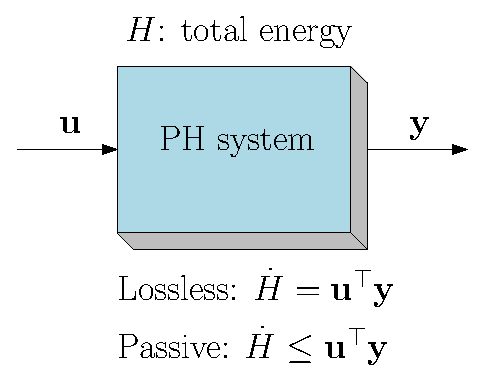
\includegraphics[width=.95\textwidth]{sketch_PH.eps}
				\end{figure}
			\end{column}
			\hspace{1cm}
			\begin{column}{.5\textwidth}
				PH systems are:
				\begin{itemize}
					\item Physically motivated;
					\item Lumped (ODEs) or distributed (PDEs);
					\item Passive (passivity based control);
					\item \textcolor{red}{Closed under interconnection (modular multiphysics modelling)};
				\end{itemize}
			\begin{block}{Necessity of numerical methods}
				To tackle complex models and for control implementation, numerical methods are needed.
			\end{block}
			
			\end{column}
		\end{columns}	
\end{frame}


\begin{frame}{State of the art and this contribution}
Discretization of port-Hamiltonian systems:
\begin{itemize}
\item Mixed finite elements for differential forms\footfullcite{golo2004hamiltonian} \footfullcite{kotyczka2018weak};
\item Spectral methods\footfullcite{moulla2012pseudo};
\item Finite differences\footfullcite{trenchant2018}.
\end{itemize}

\begin{exampleblock}{This contribution}
	Mixed finite element for hyperbolic PDEs in port-Hamiltonian form under uniform or mixed boundary conditions. 
\end{exampleblock}

\end{frame}


\section{Structure preserving discretization through mixed finite elements}


\begin{frame}{Structure preserving discretization}
	\begin{tcbraster}[raster columns=2, raster equal height]
		\begin{tcolorbox}[width=0.4\textwidth, nobeforeafter, colframe=theme,title=Infinite-dimensional pH system]%%
			PDE with boundary control:
			\begin{equation*}
				\diffp{\bm{\alpha}}{t}(\bm{x}, t) = \mathcal{J} \delta_{\bm{\alpha}} H.
			\end{equation*}
			Boundary conditions: 
			\[\textcolor{blue}{\bm{u}_\partial} = \mathcal{B}_\partial \delta_{\bm{\alpha}} H, \quad \textcolor{blue}{\bm{y}_\partial} = \mathcal{C}_\partial \delta_{\bm{\alpha}} H. \]
			Power balance (Stokes Theorem): 
			\[ \dot{H} = \displaystyle \int_{\partial \Omega} \textcolor{blue}{\bm{u}_\partial} \cdot \textcolor{blue}{\bm{y}_\partial} \d{S}.
			\]
		\end{tcolorbox} 
		\begin{tcolorbox}[width=0.4\textwidth, nobeforeafter,  colframe=theme,title=Structure-preserving discretization]%%
			Resulting ODE:
			\begin{align*}
				\dot{\bm{\alpha}}_d &= \mathbf{J} \, {\nabla {H}_d} + \mathbf{B}_\partial \textcolor{blue}{\mathbf{u}_\partial}, \\
				\textcolor{blue}{\mathbf{y}_\partial} &= \mathbf{B}_\partial^\top \,{\nabla {H}_d}.
			\end{align*}
			Discretized Hamiltonian:
			\[
			H_d := H(\bm{\alpha} \equiv \bm{\alpha}_d).
			\]
			Power balance: 
			\[ \dot{H} = \textcolor{blue}{\mathbf{u}_\partial^\top \mathbf{y}_\partial}.
			\]
		\end{tcolorbox}
	\end{tcbraster}
\end{frame}

\subsection{Uniform boundary conditions}

\begin{frame}{Underlying hypotheses of the method}
	\only<1>{
		\begin{assumption}[Partitioned structure of the pH system]
			The pH system has the partitioned form
			\begin{align*}
				\begin{aligned}
					\partial_t \begin{pmatrix}
						{\bm{\alpha}}_1 \\ {\bm{\alpha}}_2
					\end{pmatrix} &= \begin{bmatrix}
						0 & - \mathcal{L}^* \\
						\mathcal{L} & 0 \\
					\end{bmatrix}\begin{pmatrix}
						\bm{e}_1 \\ \bm{e}_2
					\end{pmatrix} , \vspace{3pt}\\
					\begin{pmatrix}
						\bm{e}_1 \\ \bm{e}_2
					\end{pmatrix} &:= \begin{pmatrix}
						\delta_{\bm{\alpha}_1}H \\ \delta_{\bm{\alpha}_2}H
					\end{pmatrix},
				\end{aligned} \qquad
				\begin{aligned}
					\bm{\alpha}_1 &\in L^2(\Omega, \mathbb{A}), 	\\
					\bm{\alpha}_2 &\in L^2(\Omega, \mathbb{B}),  \\
					\bm{e}_1 &\in H^\mathcal{L}:= \left\{\bm{u}_1 \in L^2(\Omega, \mathbb{A}) \vert \; \mathcal{L}\bm{u}_1 \in L^2(\Omega, \mathbb{B}) \right\}, 	\\
					\bm{e}_2 &\in H^{\mathcal{L}^*}:= \left\{\bm{u}_2 \in L^2(\Omega, \mathbb{B}) \vert \; \mathcal{L}^*\bm{u}_2 \in L^2(\Omega, \mathbb{A}) \right\}.
				\end{aligned}
			\end{align*}
			The  sets $\mathbb{A}, \mathbb{B}$ are Cartesian product of either scalar, vectorial or tensorial quantities.
		\end{assumption}
		Wave-like equations (e.g. linear elastic models) possess this structure  \footfullcite{joly2003variational}.
	}
	
	\only<2>{
		\begin{assumption}[Abstract integration by parts formula]
			There exists  two boundary operators $\mathcal{N}_{\partial, 1}, \; \mathcal{N}_{\partial, 2}$ such that  a general integration by parts formula holds $\forall \bm{e}_1 \in H^\mathcal{L}$ and $\forall \bm{e}_2 \in H^{\mathcal{L}^*}$
			\begin{equation*}
				\inner[L^2(\Omega, \mathbb{B})]{\bm{e}_2}{\mathcal{L}\,\bm{e}_1} - \inner[L^2(\Omega, \mathbb{A})]{\mathcal{L}^* \, \bm{e}_2}{\bm{e}_1} = \inner[\partial \Omega]{\mathcal{N}_{\partial, 1} \bm{e}_1}{\mathcal{N}_{\partial, 2} \bm{e}_2}. 
			\end{equation*}
			where $\inner[\partial \Omega]{\cdot}{\cdot}$ denotes an appropriate duality pairing.
		\end{assumption}
		
		\begin{assumption}[Uniform boundary condition]
			The boundary operators $\mathcal{B}_\partial, \, \mathcal{C}_\partial$ are then assumed to verify, in an exclusive manner, either
			\begin{equation*}
				\mathcal{B}_\partial = \begin{bmatrix}
					0 & \mathcal{N}_{\partial, 2} \\
				\end{bmatrix}, \qquad 
				\mathcal{C}_\partial = \begin{bmatrix}
					\mathcal{N}_{\partial, 1} & 0 \\
				\end{bmatrix},
			\end{equation*}
			or 
			\begin{equation*}
				\mathcal{B}_\partial = \begin{bmatrix}
					\mathcal{N}_{\partial, 1} & 0 \\
				\end{bmatrix}, \qquad \mathcal{C}_\partial = \begin{bmatrix}
					0 & \mathcal{N}_{\partial, 2} \\
				\end{bmatrix}.
			\end{equation*}
		\end{assumption}
	}
	
\end{frame}

\begin{frame}{The partitioned finite element method}
	\begin{overlayarea}{\textwidth}{.4\textheight}
		This discretization procedure represents the application of mixed finite elements to port-Hamiltonian systems:
		\vspace{.3cm}
		\setbeamercovered{transparent}
		\begin{enumerate}
			\item \only<2->{The system is written in weak form;} 
			\item \only<3-4>{An integration by parts is applied to highlight the appropriate boundary control;} \only<5>{\textcolor{red}{An integration by parts is applied to highlight the appropriate boundary control;}}
			\item \only<4->{A Galerkin method is employed to obtain a finite-dimensional system. For the approximation basis the Finite Element Method FEM (large sparse matrices) is here employed but Spectral Methods SM (small full matrices) can be used as well.}
		\end{enumerate}
	\end{overlayarea}
\end{frame}

\begin{frame}{The discretized system}
	\only<1>{
		Consider the causality 
		\begin{equation*}
			\bm{u}_\partial = \mathcal{N}_{\partial, 1} \displaystyle \bm{e}_1, \qquad  \bm{y}_\partial = \mathcal{N}_{\partial, 2} \displaystyle \bm{e}_2.
		\end{equation*}
		By integrating by parts  $\mathcal{L}$ the appropriate causality is obtained for the discretized system.
		\begin{exampleblock}{Finite dimensional system for $\bm{u}_\partial = \mathcal{N}_{\partial, 1} \displaystyle \bm{e}_1$}
			\begin{equation*}
				\begin{aligned}
					\begin{bmatrix}
						\mathbf{M}_1 & \mathbf{0} \\
						\mathbf{0} & \mathbf{M}_2 \\
					\end{bmatrix}
					\begin{pmatrix}
						\dot{\bm{\alpha}}_{d, 1} \\
						\dot{\bm{\alpha}}_{d, 2} \\
					\end{pmatrix}
					&= \begin{bmatrix}
						\mathbf{0} & \mathbf{D}_{-\mathcal{L}^*} \\
						- \mathbf{D}_{-\mathcal{L}^*}^\top & \mathbf{0} \\
					\end{bmatrix} 
					\begin{pmatrix}
						\mathbf{e}_{1} \\
						\mathbf{e}_{2} \\
					\end{pmatrix} + 
					\begin{bmatrix}
						\mathbf{0}\\
						\mathbf{B}_2\\
					\end{bmatrix}
					\mathbf{u}_\partial, \\
					\begin{bmatrix}
						\mathbf{M}_1 & \mathbf{0} \\
						\mathbf{0} & \mathbf{M}_2 \\
					\end{bmatrix}
					\begin{pmatrix}
						\mathbf{e}_{1} \\
						\mathbf{e}_{2} \\
					\end{pmatrix}
					&= \begin{pmatrix}
						\partial_{\bm{\alpha}_{d, 1}} H_d(\bm{\alpha}_d)\\
						\partial_{\bm{\alpha}_{d, 2}} H_d(\bm{\alpha}_d)\\
					\end{pmatrix}, \\
					\mathbf{M}_\partial {\mathbf{y}_\partial} &= 
					\begin{bmatrix}
						\mathbf{0} & \mathbf{B}_2^\top 
					\end{bmatrix}\begin{pmatrix}
						\mathbf{e}_{1} \\
						\mathbf{e}_{2} \\
					\end{pmatrix}.
				\end{aligned}
			\end{equation*}
		\end{exampleblock}
	}
	
	\only<2>{
		Consider the causality
		\begin{equation*}
			\bm{u}_\partial = \mathcal{N}_{\partial, 2} \displaystyle \bm{e}_2, \qquad  \bm{y}_\partial = \mathcal{N}_{\partial, 1} \displaystyle \bm{e}_1.
		\end{equation*}
		By integrating by parts  $-\mathcal{L}^*$ the appropriate causality is obtained for the discretized system.
		\begin{exampleblock}{Finite dimensional system for $\bm{u}_\partial = \mathcal{N}_{\partial, 2} \displaystyle \bm{e}_2$}
			\begin{equation*}
				\begin{aligned}
					\begin{bmatrix}
						\mathbf{M}_1 & \mathbf{0} \\
						\mathbf{0} & \mathbf{M}_2 \\
					\end{bmatrix}
					\begin{pmatrix}
						\dot{\bm{\alpha}}_{d, 1} \\
						\dot{\bm{\alpha}}_{d, 2} \\
					\end{pmatrix}
					&= \begin{bmatrix}
						\mathbf{0} & - \mathbf{D}_{\mathcal{L}}^\top \\
						\mathbf{D}_{\mathcal{L}} & \mathbf{0} \\
					\end{bmatrix} 
					\begin{pmatrix}
						\mathbf{e}_{1} \\
						\mathbf{e}_{2} \\
					\end{pmatrix} + 
					\begin{bmatrix}
						\mathbf{B}_1\\
						\mathbf{0}\\
					\end{bmatrix}
					\mathbf{u}_\partial, \\
					\begin{bmatrix}
						\mathbf{M}_1 & \mathbf{0} \\
						\mathbf{0} & \mathbf{M}_2 \\
					\end{bmatrix}
					\begin{pmatrix}
						\mathbf{e}_{1} \\
						\mathbf{e}_{2} \\
					\end{pmatrix}
					&= \begin{bmatrix}
						\partial_{\bm{\alpha}_{d, 1}} H_d(\bm{\alpha}_d)\\
						\partial_{\bm{\alpha}_{d, 2}} H_d(\bm{\alpha}_d)\\
					\end{bmatrix}, \\
					\mathbf{M}_\partial {\mathbf{y}_\partial} &= \begin{bmatrix}
						\mathbf{B}_1^\top & \mathbf{0}
					\end{bmatrix}\begin{pmatrix}
						\mathbf{e}_{1} \\
						\mathbf{e}_{2} \\
					\end{pmatrix}.
				\end{aligned}
			\end{equation*}
		\end{exampleblock}
	}
	
\end{frame}

\begin{frame}{Discrete power balance}
	The power balance
	\begin{equation*}
		\dot{H}_d = \partial_{\bm{\alpha}_{d, 1}}^\top H_d(\bm{\alpha}_d) \dot{\bm{\alpha}}_{d, 1} + \partial_{\bm{\alpha}_{d, 2}}^\top H_d(\bm{\alpha}_d) \dot{\bm{\alpha}}_{d, 2}
	\end{equation*}
	mimics the continuous one.
	
	\begin{exampleblock}{Causality $\bm{u}_\partial = \mathcal{N}_{\partial, 1} \displaystyle \bm{e}_1$}
		
		\begin{equation*}
			\begin{aligned}
				\dot{H}_d &= \mathbf{e}_{1}^\top \mathbf{D}_{-\mathcal{L}^*} \mathbf{e}_{2} - \mathbf{e}_{2}^\top \mathbf{D}_{-\mathcal{L}^*}^\top \mathbf{e}_{1} + \mathbf{e}_{2}^\top \mathbf{B}_2 \mathbf{u}_\partial, \\
				& = \mathbf{y}_\partial^\top \mathbf{M}_\partial \mathbf{u}_\partial
			\end{aligned}
		\end{equation*}
		
	\end{exampleblock}
	
	\begin{exampleblock}{Causality $\bm{u}_\partial = \mathcal{N}_{\partial, 2} \displaystyle \bm{e}_2$}
		
		\begin{equation*}
			\begin{aligned}
				\dot{H}_d &= - \mathbf{e}_{1}^\top \mathbf{D}_{\mathcal{L}}^\top \mathbf{e}_{2} + \mathbf{e}_{2}^\top \mathbf{D}_{\mathcal{L}} \mathbf{e}_{1} + \mathbf{e}_{1}^\top \mathbf{B}_1 \mathbf{u}_\partial, \\
				& = \mathbf{y}_\partial^\top \mathbf{M}_\partial \mathbf{u}_\partial.
			\end{aligned}
		\end{equation*}
		
	\end{exampleblock}
	
\end{frame}


\subsection{The linear case}

\begin{frame}
	\begin{assumption}[Quadratic separable Hamiltonian]
		The Hamiltonian is assumed to be a positive quadratic separable functional in $\bm{\alpha}_1, \, \bm{\alpha}_2$ 
		\begin{equation*}
			H = \frac{1}{2} \inner[L^2(\Omega, \mathbb{A})]{\bm{\alpha}_{1}}{\mathcal{Q}_1\bm{\alpha}_{1}} + \frac{1}{2} \inner[L^2(\Omega, \mathbb{B})]{\bm{\alpha}_{2}}{\mathcal{Q}_2\bm{\alpha}_{2}},
		\end{equation*}
		where $\mathcal{Q}_1, \, \mathcal{Q}_2$ are positive symmetric bounded operators
		\begin{equation*}
			m_1 \bm{I}_\mathbb{A} \le\mathcal{Q}_1 \le M_1 \bm{I}_\mathbb{A}, \qquad  m_2 \bm{I}_\mathbb{B} \le \mathcal{Q}_2 \le M_2 \bm{I}_\mathbb{B}, \qquad m_1>0, \ m_2>0, \ M_1>0, \ M_2>0.
		\end{equation*} 
	\end{assumption}
	
	
	\begin{exampleblock}{PH linear system}
		\begin{equation*}
			\begin{bmatrix}
				\mathcal{M}_1 & 0 \\
				0 & \mathcal{M}_2 \\
			\end{bmatrix}
			\partial_t \begin{pmatrix}
				\bm{e}_1 \\ \bm{e}_2
			\end{pmatrix} = \begin{bmatrix}
				0 &  - \mathcal{L}^* \\
				\mathcal{L} & 0 \\
			\end{bmatrix}\begin{pmatrix}
				\bm{e}_1 \\ \bm{e}_2
			\end{pmatrix} , \qquad \begin{aligned}
				\bm{e}_1 &\in H^{\mathcal{L}}, 	\\
				\bm{e}_2 &\in H^{\mathcal{L}^*},
			\end{aligned}
		\end{equation*}
		where $\mathcal{M}_1:=\mathcal{Q}_1^{-1},\; \mathcal{M}_2:=\mathcal{Q}_2^{-1}$. \textbf{Constitutive laws} have been included in the dynamics.
	\end{exampleblock}
	
\end{frame}

\begin{frame}{The linear discretized system}
	\begin{exampleblock}{Finite dimensional system for $\bm{u}_\partial = \mathcal{N}_{\partial, 1} \displaystyle \bm{e}_1, \;  \bm{y}_\partial = \mathcal{N}_{\partial, 2} \displaystyle \bm{e}_2$}
		\begin{equation*}
			\begin{aligned}
				\begin{bmatrix}
					\mathbf{M}_{\mathcal{M}_1} & \mathbf{0} \\
					\mathbf{0} & \mathbf{M}_{\mathcal{M}_2} \\
				\end{bmatrix}
				\begin{pmatrix}
					\dot{\mathbf{e}}_{1} \\
					\dot{\mathbf{e}}_{2} \\
				\end{pmatrix}
				&= \begin{bmatrix}
					\mathbf{0} & \mathbf{D}_{-\mathcal{L}^*} \\
					- \mathbf{D}_{-\mathcal{L}^*}^\top & \mathbf{0} \\
				\end{bmatrix} 
				\begin{pmatrix}
					\mathbf{e}_{1} \\
					\mathbf{e}_{2} \\
				\end{pmatrix} + 
				\begin{bmatrix}
					\mathbf{0}\\
					\mathbf{B}_2\\
				\end{bmatrix}
				\mathbf{u}_\partial, \\
				\mathbf{M}_\partial {\mathbf{y}_\partial} &= 
				\begin{bmatrix}
					\mathbf{0} & \mathbf{B}_2^\top 
				\end{bmatrix}\begin{pmatrix}
					\mathbf{e}_{1} \\
					\mathbf{e}_{2} \\
				\end{pmatrix}.
			\end{aligned}
		\end{equation*}
	\end{exampleblock}
	
	\begin{exampleblock}{Finite dimensional system for $\bm{u}_\partial = \mathcal{N}_{\partial, 2} \displaystyle \bm{e}_2, \; \bm{y}_\partial = \mathcal{N}_{\partial, 1} \displaystyle \bm{e}_1$}
		\begin{equation*}
			\begin{aligned}
				\begin{bmatrix}
					\mathbf{M}_{\mathcal{M}_1} & \mathbf{0} \\
					\mathbf{0} & \mathbf{M}_{\mathcal{M}_2} \\
				\end{bmatrix}
				\begin{pmatrix}
					\dot{\mathbf{e}}_{1} \\
					\dot{\mathbf{e}}_{2} \\
				\end{pmatrix}
				&= \begin{bmatrix}
					\mathbf{0} & - \mathbf{D}_{\mathcal{L}}^\top \\
					\mathbf{D}_{\mathcal{L}} & \mathbf{0} \\
				\end{bmatrix} 
				\begin{pmatrix}
					\mathbf{e}_{1} \\
					\mathbf{e}_{2} \\
				\end{pmatrix} + 
				\begin{bmatrix}
					\mathbf{B}_1\\
					\mathbf{0}\\
				\end{bmatrix}
				\mathbf{u}_\partial, \\
				\mathbf{M}_\partial {\mathbf{y}_\partial} &= \begin{bmatrix}
					\mathbf{B}_1^\top & \mathbf{0}
				\end{bmatrix}\begin{pmatrix}
					\mathbf{e}_{1} \\
					\mathbf{e}_{2} \\
				\end{pmatrix}.
			\end{aligned}
		\end{equation*}
	\end{exampleblock}
	
\end{frame}

\begin{frame}{Power balance}
	The power balance 
	\begin{equation*}
		\dot{H}_d = \mathbf{e}_1^\top \mathbf{M}_{\mathcal{M}_1} \dot{\mathbf{e}}_{1} + \mathbf{e}_2^\top \mathbf{M}_{\mathcal{M}_2} \dot{\mathbf{e}}_{2} 
	\end{equation*}
	mimics the continuous one.
	
	\begin{exampleblock}{Causality $\bm{u}_\partial = \mathcal{N}_{\partial, 1} \displaystyle \bm{e}_1$}
		
		\begin{equation*}
			\begin{aligned}
				\dot{H}_d &= \mathbf{e}_{1}^\top \mathbf{D}_{-\mathcal{L}^*} \mathbf{e}_{2} - \mathbf{e}_{2}^\top \mathbf{D}_{-\mathcal{L}^*}^\top \mathbf{e}_{1} + \mathbf{e}_{2}^\top \mathbf{B}_2 \mathbf{u}_\partial, \\
				& = \mathbf{y}_\partial^\top \mathbf{M}_\partial \mathbf{u}_\partial
			\end{aligned}
		\end{equation*}
		
	\end{exampleblock}
	
	\begin{exampleblock}{Causality $\bm{u}_\partial = \mathcal{N}_{\partial, 2} \displaystyle \bm{e}_2$}
		
		\begin{equation*}
			\begin{aligned}
				\dot{H}_d 	&= - \mathbf{e}_{1}^\top \mathbf{D}_{\mathcal{L}}^\top \mathbf{e}_{2} + \mathbf{e}_{2}^\top \mathbf{D}_{\mathcal{L}} \mathbf{e}_{1} + \mathbf{e}_{1}^\top \mathbf{B}_1 \mathbf{u}_\partial, \\
				& = \mathbf{y}_\partial^\top \mathbf{M}_\partial \mathbf{u}_\partial.
			\end{aligned}
		\end{equation*}
		
	\end{exampleblock}
\end{frame}


\subsection{Mixed boundary conditions}

\begin{frame}{Mixed boundary conditions (linear system)}
	
	Consider now the following boundary-controlled linear pH system in co-energy form 
	\begin{columns}
		\begin{column}{0.6\textwidth}
			\begin{align*}
				\begin{bmatrix}
					\mathcal{M}_1 & 0 \\
					0 & \mathcal{M}_2 \\
				\end{bmatrix}
				\partial_t \begin{pmatrix}
					\bm{e}_1 \\ \bm{e}_2
				\end{pmatrix} &= \begin{bmatrix}
					0 &- \mathcal{L}^* \\
					\mathcal{L} & 0 \\
				\end{bmatrix}\begin{pmatrix}
					\bm{e}_1 \\ \bm{e}_2
				\end{pmatrix}, \\
				\begin{pmatrix}
					\bm{u}_{\partial, 1}\\
					\bm{u}_{\partial, 2}\\
				\end{pmatrix} &= \begin{bmatrix}
					\mathcal{N}_{\partial, 1}^{\Gamma_1} & 0\\
					0 & \mathcal{N}_{\partial, 2}^{\Gamma_2} \\
				\end{bmatrix} \begin{pmatrix}
					\bm{e}_1 \\ \bm{e}_2
				\end{pmatrix}, \\
				\begin{pmatrix}
					\bm{y}_{\partial, 1}\\
					\bm{y}_{\partial, 2}\\
				\end{pmatrix} &= \begin{bmatrix}
					0 & \mathcal{N}_{\partial, 2}^{\Gamma_1} \\
					\mathcal{N}_{\partial, 1}^{\Gamma_2} & 0\\
				\end{bmatrix} \begin{pmatrix}
					\bm{e}_1 \\ \bm{e}_2
				\end{pmatrix}.
			\end{align*}
		\end{column}
		\begin{column}{0.4\textwidth}
			\begin{figure}[tb]
				\centering
				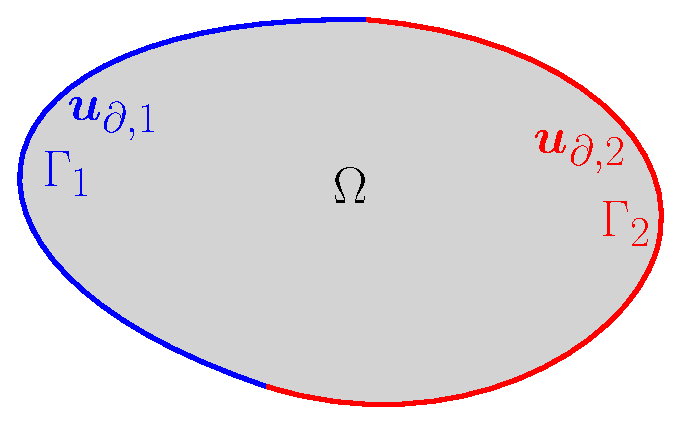
\includegraphics[width=0.9\columnwidth]{pfem/bound_part.eps}
			\end{figure}
		\end{column}
	\end{columns}
	
	\vspace{1cm}
	The operator $\mathcal{N}_{\partial, *}^{\Gamma_\circ}$ with $*, \circ \in \{1, 2\}$ represents the restriction of operator $\mathcal{N}_{\partial, *}$ over the subset $\Gamma_\circ \subset \partial\Omega$.
\end{frame}


\begin{frame}{Lagrange multiplier method}
	A Lagrange multiplier can be introduced to include the input that does not explicitly appear in the weak formulation, i.e. to enforce the essential boundary condition. 
	\only<1>{
		\setbeamercolor{block title}{bg=yellow, fg=black}
		\begin{block}{Integration by parts of $-\mathcal{L}^*$ ($\textcolor{blue}{\bm{\lambda}_{\partial, 1}}=\textcolor{blue}{\bm{y}_{\partial, 1}}$) }
			\begin{equation*}
				\begin{aligned}
					\mathrm{Diag}
					\begin{bmatrix}
						\mathbf{M}_{\mathcal{M}_1}\\
						\mathbf{M}_{\mathcal{M}_2}\\
						\mathbf{0}\\
					\end{bmatrix}
					\begin{pmatrix}
						\dot{\mathbf{e}}_{1} \\
						\dot{\mathbf{e}}_{2} \\
						\textcolor{blue}{\dot{\bm{\lambda}}_{\partial, 1}} \\
					\end{pmatrix}
					&= \begin{bmatrix}
						\mathbf{0} & - \mathbf{D}_{\mathcal{L}}^\top & \mathbf{B}_{1, \textcolor{blue}{\Gamma_1}}\\
						\mathbf{D}_{\mathcal{L}} & \mathbf{0} & \mathbf{0} \\
						-\mathbf{B}_{1, \textcolor{blue}{\Gamma_1}}^\top & \mathbf{0} & \mathbf{0} \\
					\end{bmatrix} 
					\begin{pmatrix}
						\mathbf{e}_{1} \\
						\mathbf{e}_{2} \\
						\textcolor{blue}{\bm{\lambda}_{\partial, 1}} \\
					\end{pmatrix} + 
					\begin{bmatrix}
						\mathbf{0} & \mathbf{B}_{1, \textcolor{red}{\Gamma_2}} \\
						\mathbf{0} & \mathbf{0} \\
						\mathbf{M}_{\partial, 1} & \mathbf{0} \\
					\end{bmatrix}
					\begin{bmatrix}
						\textcolor{blue}{\mathbf{u}_{\partial, 1}} \\
						\textcolor{red}{\mathbf{u}_{\partial, 2}} \\
					\end{bmatrix}, \\
					\begin{bmatrix}
						\mathbf{M}_{\partial, 1} & \mathbf{0} \\
						\mathbf{0} & \mathbf{M}_{\partial, 2} \\
					\end{bmatrix}
					\begin{pmatrix}
						\textcolor{blue}{\mathbf{y}_{\partial, 1}} \\
						\textcolor{red}{\mathbf{y}_{\partial, 2}} \\
					\end{pmatrix}
					&= \begin{bmatrix}
						\mathbf{0} & \mathbf{0} & \mathbf{M}_{\partial, 1} \\
						\mathbf{B}_{1, \textcolor{red}{\Gamma_2}}^\top & \mathbf{0} & \mathbf{0} \\
					\end{bmatrix}\begin{pmatrix}
						\mathbf{e}_{1} \\
						\mathbf{e}_{2} \\
						\textcolor{blue}{\bm{\lambda}_{\partial, 1}} \\
					\end{pmatrix}.
				\end{aligned}
			\end{equation*}
		\end{block}	
	}
	
	
	\only<2>{
		\setbeamercolor{block title}{bg=yellow, fg=black}
		\begin{block}{Integration by parts of $\mathcal{L}$ ($\textcolor{red}{\bm{\lambda}_{\partial, 2}} = \textcolor{red}{\bm{y}_{\partial, 2}}$)}
			\begin{equation*}
				\begin{aligned}
					\mathrm{Diag}
					\begin{bmatrix}
						\mathbf{M}_{\mathcal{M}_1}\\
						\mathbf{M}_{\mathcal{M}_2}\\
						\mathbf{0}\\
					\end{bmatrix}
					\begin{pmatrix}
						\dot{\mathbf{e}}_{1} \\
						\dot{\mathbf{e}}_{2} \\
						\textcolor{red}{\dot{\bm{\lambda}}_{\partial, 2}} \\
					\end{pmatrix}
					&= \begin{bmatrix}
						\mathbf{0} & \mathbf{D}_ {-\mathcal{L}^*} & \mathbf{0}\\
						- \mathbf{D}_ {-\mathcal{L}^*}^\top & \mathbf{0} & \mathbf{B}_{2, \textcolor{red}{\Gamma_2}} \\
						\mathbf{0} & -\mathbf{B}_{2, \textcolor{red}{\Gamma_2}}^\top & \mathbf{0}  \\
					\end{bmatrix} 
					\begin{pmatrix}
						\mathbf{e}_{1} \\
						\mathbf{e}_{2} \\
						\textcolor{red}{\bm{\lambda}_{\partial, 2}} \\
					\end{pmatrix} + 
					\begin{bmatrix}
						\mathbf{0} & \mathbf{0} \\
						\mathbf{B}_{2, \textcolor{blue}{\Gamma_1}} & \mathbf{0} \\
						\mathbf{0} & \mathbf{M}_{\partial, 2} \\
					\end{bmatrix}
					\begin{bmatrix}
						\textcolor{blue}{\mathbf{u}_{\partial, 1}} \\
						\textcolor{red}{\mathbf{u}_{\partial, 2}} \\
					\end{bmatrix}, \\
					\begin{bmatrix}
						\mathbf{M}_{\partial, 1} & \mathbf{0} \\
						\mathbf{0} & \mathbf{M}_{\partial, 2} \\
					\end{bmatrix}
					\begin{pmatrix}
						\textcolor{blue}{\mathbf{y}_{\partial, 1}} \\
						\textcolor{red}{\mathbf{y}_{\partial, 2}} \\
					\end{pmatrix}
					&= \begin{bmatrix}
						\mathbf{0} & \mathbf{B}_{2, \textcolor{blue}{\Gamma_1}}^\top & \mathbf{0} \\
						\mathbf{0} & \mathbf{0} & \mathbf{M}_{\partial, 2} \\
					\end{bmatrix}\begin{pmatrix}
						\mathbf{e}_{1} \\
						\mathbf{e}_{2} \\
						\textcolor{red}{\bm{\lambda}_{\partial, 2}} \\
					\end{pmatrix}.
				\end{aligned}
			\end{equation*}
		\end{block}
	}
	A pH differential-algebraic system is obtained in this case (pHDAE).
\end{frame}

\begin{frame}{Power balance}
	The energy balance
	\begin{equation*}
		\dot{H}_d = \mathbf{e}_1^\top \mathbf{M}_{\mathcal{M}_1} \dot{\mathbf{e}}_1 + \mathbf{e}_2^\top \mathbf{M}_{\mathcal{M}_2} \dot{\mathbf{e}}_2
	\end{equation*}
	mimics the continuous counterpart.
	\begin{exampleblock}{Integration by parts of $-\mathcal{L}^*$ ($\bm{\lambda}_{\partial, 1} = \bm{u}_{\partial, 1}$)}
		\begin{equation*}
			\begin{aligned}
				\dot{H}_d &= -\mathbf{e}_1^\top \mathbf{D}_\mathcal{L}^\top {\mathbf{e}}_2 + \mathbf{e}_2^\top\mathbf{D}_\mathcal{L} {\mathbf{e}}_1 + \mathbf{e}_1^\top (\mathbf{B}_{1, \Gamma_1} \bm{\lambda}_{\partial, 1} + \mathbf{B}_{1, \Gamma_2} \mathbf{u}_{\partial, 2} ), \\
				&= \mathbf{y}_{\partial, 1}^\top \mathbf{M}_{\partial, 1} \mathbf{u}_{\partial, 1} + \mathbf{y}_{\partial, 2}^\top \mathbf{M}_{\partial, 2} \mathbf{u}_{\partial, 2}. 
			\end{aligned}
		\end{equation*}
	\end{exampleblock}
	\begin{exampleblock}{Integration by parts of $\mathcal{L}$ ($\bm{\lambda}_{\partial, 2} = \bm{u}_{\partial, 2}$)}
		\begin{equation*}
			\begin{aligned}
				\dot{H}_d &= \mathbf{e}_1^\top \mathbf{D}_{-\mathcal{L}^*}^\top {\mathbf{e}}_2 - \mathbf{e}_2^\top\mathbf{D}_{-\mathcal{L}^*} {\mathbf{e}}_1 + \mathbf{e}_2^\top (\mathbf{B}_{2, \Gamma_2} \bm{\lambda}_{\partial, 2} + \mathbf{B}_{2, \Gamma_1} \mathbf{u}_{\partial, 1} ), \\
				&= \mathbf{y}_{\partial, 1}^\top \mathbf{M}_{\partial, 1} \mathbf{u}_{\partial, 1} + \mathbf{y}_{\partial, 2}^\top \mathbf{M}_{\partial, 2} \mathbf{u}_{\partial, 2}. 
			\end{aligned}
		\end{equation*}
	\end{exampleblock}
\end{frame}



\section{Applications}

\subsection{Boundary control of the irrotational shallow water equations}

\begin{frame}{Irrotational shallow water equations}
	
The Hamiltonian is a non-quadratic and non-separable functional
\begin{equation*}
		H(\alpha_h, \bm{\alpha}_v) = \energy{\frac{1}{\rho} \alpha_h \norm{\bm{\alpha}_v}^2 + \rho g \alpha_h^2}.
\end{equation*}


\begin{columns}
	
	\begin{column}{.45\textwidth}
		Variables: 
		\begin{itemize}
			\item $\alpha_h$ the fluid height;
			\item $\bm{\alpha}_v$ the linear momentum;
		\end{itemize}
	\end{column}
	
	\begin{column}{.45\textwidth}
		Parameters:
		\begin{itemize}
			\item $\rho$ density;
			\item $g$ gravity acceleration
		\end{itemize}
	\end{column}
	
\end{columns}

\vspace{.5cm}
	
	Dynamics:
	\begin{equation*} 
		\begin{aligned}
			\diffp{}{t}
			\begin{pmatrix}
				\alpha_h \\
				\bm{\alpha}_v \\
			\end{pmatrix} &= 
			\begin{bmatrix}
				0 & -\div \\
				-\grad & \bm{0}
			\end{bmatrix}
			\begin{pmatrix}
				e_h\\
				\bm{e}_v\\
			\end{pmatrix}, \qquad (x,y) \in \Omega = \{x^2 + y^2 \le R \}, \\
			\begin{pmatrix}
				e_h\\
				\bm{e}_v\\
			\end{pmatrix} &= \begin{pmatrix}
				\delta_{\alpha_h} H\\
				\delta_{\bm{\alpha}_v} H\\
			\end{pmatrix} = 
			\begin{pmatrix}
				\frac{1}{2 \rho} \norm{\bm{\alpha}_v}^2 + \rho g \alpha_h \\
				\frac{1}{\rho} \alpha_h \bm{\alpha}_v
			\end{pmatrix}, 
		\end{aligned}
	\end{equation*}
	
\end{frame}


\begin{frame}{Proportional control law}
\begin{columns}	
\begin{column}{.45\textwidth}
Consider a uniform Neumann bc
\begin{equation*}
	{u}_\partial = - \bm{e}_v \cdot \bm{n}\vert_{\partial\Omega}.
\end{equation*}
\end{column}
\begin{column}{.45\textwidth}
Conjugated output
\begin{equation*}
	{y}_\partial = {e}_h\vert_{\partial\Omega}.
\end{equation*}
\end{column}
\end{columns}
	
	
\begin{block}{Proportional control: La Salle argument}
Proportional control for stabilization around a given fluid height $h^{\text{des}}$
\begin{equation*}
	u_\partial = -k (y_\partial - y_\partial^{\text{des}}), \qquad y_\partial^{\text{des}}= \rho g h^{\text{des}}, \quad k>0.
\end{equation*}
The control law ensures that the Lyapunov functional
\begin{equation*}
	V = \frac{1}{2} \int_{\Omega}\left\{\frac{1}{2} \rho g (\alpha_h - h^{\text{des}})^2 + \frac{1}{2\rho} \alpha_h \norm{\bm{\alpha}_v}^2 \right\} d\Omega \ge 0,
\end{equation*}
has negative semi definite time derivative
\begin{equation*}
	\dot{V} = -k \int_{\partial \Omega}\left({y}_\partial - {y}_\partial^{\text{des}} \right)^2 \d{\Gamma} \le 0.
\end{equation*}
\end{block}

\end{frame}

\begin{frame}{Discretization strategy}
	\begin{itemize}
		\item The $\div$ operator is integrated by parts to highlight the appropriate the Neumann boundary control.
		\item \fenics is used to generate the matrices.
	\end{itemize}
	
	\begin{table}[th]
		\centering
		\begin{tabular}{|c|c|}
			\hline 
			\multicolumn{2}{|c|}{Parameters} \\ 
			\hline 
			$\rho$ & $1000\; \mathrm{[kg \cdot m^3]}$ \\ 
			$g$& $10\; \mathrm{[m/s^2]}$ \\ 
			$R$& $1\; \mathrm{[m]}$\\ 
			$h^{\text{des}}$& $1\; \mathrm{[m]}$ \\ 
			\hline 
		\end{tabular} \hspace{.3cm}
		\begin{tabular}{|c|c|}
			\hline 
			\multicolumn{2}{|c|}{Simulation Settings} \\
			\hline 
			Integrator & Runge-Kutta 45 \\
			N$_{\text{dof}}^\circ$ & $3973$ \\
			FE spaces & ($\alpha_h\approx$ CG$_1$) $\times$ ($\bm{\alpha}_v\approx$ DG$_0$) $\times$ ($u_\partial\approx$ DG$_0$)\\
			$t_{\text{end}}$ & $3\; \mathrm{[s]}$\\ 
			\hline 
		\end{tabular} 
	\end{table}
	\vspace{.5cm}
	\begin{equation*}
		\text{Control parameter} \qquad 
		k = 
		\begin{cases}
			0, \quad & \forall t < 0.5 \, [\mathrm{s}], \\
			10^{-3}, \quad & \textcolor{red}{\forall t \ge 0.5} \, [\mathrm{s}].
		\end{cases}
	\end{equation*}
	
\end{frame}

\begin{frame}{Results irrotational SWE}
	
	\only<1>{
		\begin{center}
			\includemedia[
			label=vidDam,
			addresource=/home/andrea/Videos/Videos_defense/Saint_Venant_nobar.mp4,
			activate=pageopen,
			width=10cm, height=5cm,
			flashvars={
				source=/home/andrea/Videos/Videos_defense/Saint_Venant_nobar.mp4
				&loop=true
			}
			]{}{VPlayer.swf}
			
			\mediabutton[
			mediacommand=vidDam:playPause,
			]{\fbox{Play/Pause}}
			
			\begin{equation*}
				\text{Control parameter} \qquad 
				k = 
				\begin{cases}
					0, \quad & \forall t < 0.5 \, [\mathrm{s}], \\
					10^{-3}, \quad & \textcolor{red}{\forall t \ge 0.5} \, [\mathrm{s}].
				\end{cases}
			\end{equation*}
		\end{center}
	}
	
	\only<2>{
		\begin{center}
			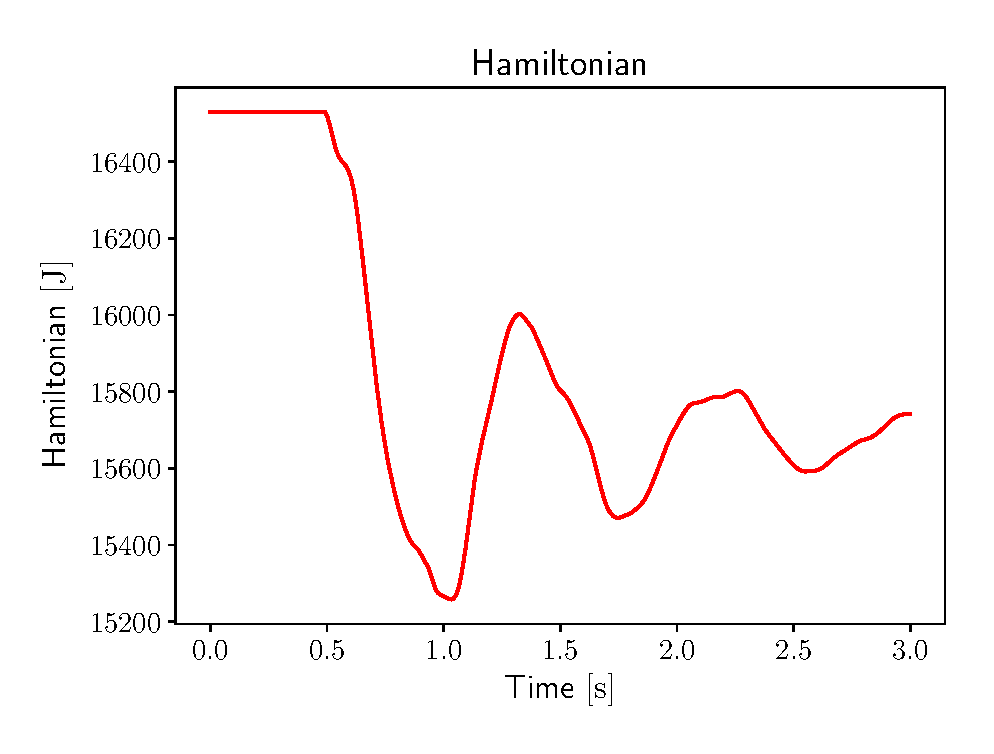
\includegraphics[width=0.48\textwidth]{bs_SWE/Hamiltonian.eps}
			\includegraphics[width=0.48\textwidth]{bs_SWE/Lyapunov.eps}
		\end{center}
	}
\end{frame}


\subsection{Boundary control of the cantilever Kirchhoff plate}

\begin{frame}{Cantilever Kirchhoff plate}
		
The Hamiltonian is a  quadratic functional (linear case), hence a co-energy formulation is used
\begin{equation*}
	H(e_w, \bm{E}_\kappa) = \energy{\rho h e_w^2 + \bm{\mathcal{D}}_b^{-1}(\bm{E}_\kappa) \cddot \bm{E}_\kappa}, \where \bm{A} \cddot \bm{B} = \sum_{ij} A_{ij}B_{ij}.
\end{equation*}


\begin{columns}
	
	\begin{column}{.45\textwidth}
		Variables: 
		\begin{itemize}
			\item $e_w$ the vertical velocity;
			\item $\bm{E}_\kappa$ the bending stress tensor;
		\end{itemize}
	\end{column}
	
	\begin{column}{.45\textwidth}
		Parameters:
		\begin{itemize}
			\item $\rho$ density, $h$ plate thickness;
			\item $\bm{\mathcal{D}}_b^{-1}$ the bending compliance tensor 
		\end{itemize}
	\end{column}
	
\end{columns}

\vspace{.5cm}
	
\begin{equation*}
	\begin{bmatrix}
		\rho h & 0 \\ 
		\bm{0} & \bm{\mathcal{D}}_b^{-1} \\
	\end{bmatrix}
	\diffp{}{t}
	\begin{pmatrix}
		e_w \\ \bm{E}_\kappa \\
	\end{pmatrix} = 
	\begin{bmatrix}
		0 & -\div\Div \\ 
		\Hess & \bm{0} \\
	\end{bmatrix}
	\begin{pmatrix}
		e_w \\ \bm{E}_\kappa \\
	\end{pmatrix} \qquad (x, y) \in \Omega = [0, 1]\times[0,1],
\end{equation*}
	
\end{frame}

\begin{frame}{Damping injection control strategy}
Consider mixed Dirichlet homogeneous conditions and Neumann boundary control
\begin{align*}
	\begin{aligned}
		e_w|_{\Gamma_D} &= 0, \\
		\partial_x e_w|_{\Gamma_D} &= 0, \\
	\end{aligned} \qquad {\Gamma_D} = \left\{x = 0 \right\}, \qquad
	\begin{aligned}
		u_{\partial, q} & = \widetilde{q}_n|_{\Gamma_N},\\
		u_{\partial, m} &= M_{nn}|_{\Gamma_N}.\\
	\end{aligned} \qquad {\Gamma_N} = \left\{y = 0 \cup x=1 \cup y=1 \right\}.
\end{align*}
where $M_{nn}$ is the flexural moment and $\widetilde{q}_n$ is the effective shear force. \vspace{.5cm}
\begin{columns}
	\setlength{\abovedisplayskip}{5pt}
	\setlength{\belowdisplayskip}{5pt}
	\begin{column}{.5\textwidth}
		The corresponding boundary outputs read
		\begin{equation*}
			\begin{aligned}
				y_{\partial, q} &= e_w|_{\Gamma_N}, \\
				y_{\partial, m} &=\partial_{\bm{n}} e_w|_{\Gamma_N}.
			\end{aligned}
		\end{equation*}
		
		The following control law stabilizes the system\footnotemark
		\begin{equation*}
			\begin{aligned}
				u_{\partial, q} & = - k y_{\partial, q}, \\
				u_{\partial, m} & = - k y_{\partial, m}, \\
			\end{aligned} \qquad k>0.
		\end{equation*}
		
	\end{column}
	
	\begin{column}{.5\textwidth}
		\begin{figure}[b]
			\centering
			\includegraphics[width=0.9\columnwidth]{bs_Kirchh/plate_controlled.eps}
		\end{figure}
	\end{column}
\end{columns}

\footcitetext{lagnese1989}
\end{frame}


\begin{frame}{Discretization strategy}
	\begin{itemize}
		\item The $\div\Div$ operator is integrated by parts twice to enforce weekly the Neumann bc.
		\item The \firedrake library is used to generate the matrices.
		\item The Dirichlet condition is imposed weakly through a Lagrange multiplier (strong imposition of boundary conditions for $H^2$ conforming elements is not trivial \footfullcite{kirby2019}).
	\end{itemize} 
	
	\begin{table}[t]
		\centering
		\begin{tabular}{|c|c|}
			\hline 
			\multicolumn{2}{|c|}{Plate Parameters} \\ 
			\hline 
			$E$ & $70\; \mathrm{[GPa]}$ \\ 
			$\rho$ & $2700\; \mathrm{[kg \cdot m^3]}$ \\ 
			$\nu$& $0.35$ \\ 
			$h/L$& $0.05$ \\ 
			$L_x = L_y$& $1\; \mathrm{[m]}$\\ 
			\hline 
		\end{tabular} \hspace{.1cm}
		\begin{tabular}{|c|c|}
			\hline 
			\multicolumn{2}{|c|}{Simulation Settings} \\
			\hline 
			Integrator & St\"ormer-Verlet \\
			$\Delta t $ & $1 \; \mathrm{[\mu s]}$ \\  
			N$_{\text{dof}}^\circ$ & $2574$ \\
			FE spaces & ($e_w \approx $ Argyris) $\times$ ($\bm{E}_\kappa \approx$ DG$_3$) $\times$ ($\bm{\lambda} \approx$ CG$_2$)\\
			$t_{\text{end}}$ & $5\; \mathrm{[s]}$\\ 
			\hline 
		\end{tabular} 
	\end{table}
	
	\begin{equation*}
		\text{Control parameter} \qquad 
		k = 
		\begin{cases}
			0, \quad &\forall t < 1 \, [\mathrm{s}], \\
			10, \quad & \textcolor{red}{\forall t \ge 1} \, [\mathrm{s}].
		\end{cases}
	\end{equation*}
	
	
\end{frame}

\begin{frame}{Results cantilever Kirchoff plate}
	\only<1>{
		\begin{center}
			\includemedia[
			label=vidDam,
			addresource=/home/andrea/Videos/Videos_defense/Kirchh_Damped_rendered.mp4,
			activate=pageopen,
			width=10cm, height=5cm,
			flashvars={
				source=/home/andrea/Videos/Videos_defense/Kirchh_Damped_rendered.mp4
				&loop=true
			}
			]{}{VPlayer.swf}
			
			\mediabutton[
			mediacommand=vidDam:playPause,
			]{\fbox{Play/Pause}}
			
			\begin{equation*}
				\text{Control parameter} \qquad 
				k = 
				\begin{cases}
					0, \quad &\forall t < 1 \, [\mathrm{s}], \\
					10, \quad & \textcolor{red}{\forall t \ge 1} \, [\mathrm{s}].
				\end{cases}
			\end{equation*}
		\end{center}
	}
	\only<2>{
		\begin{figure}[htb]
			\centering
			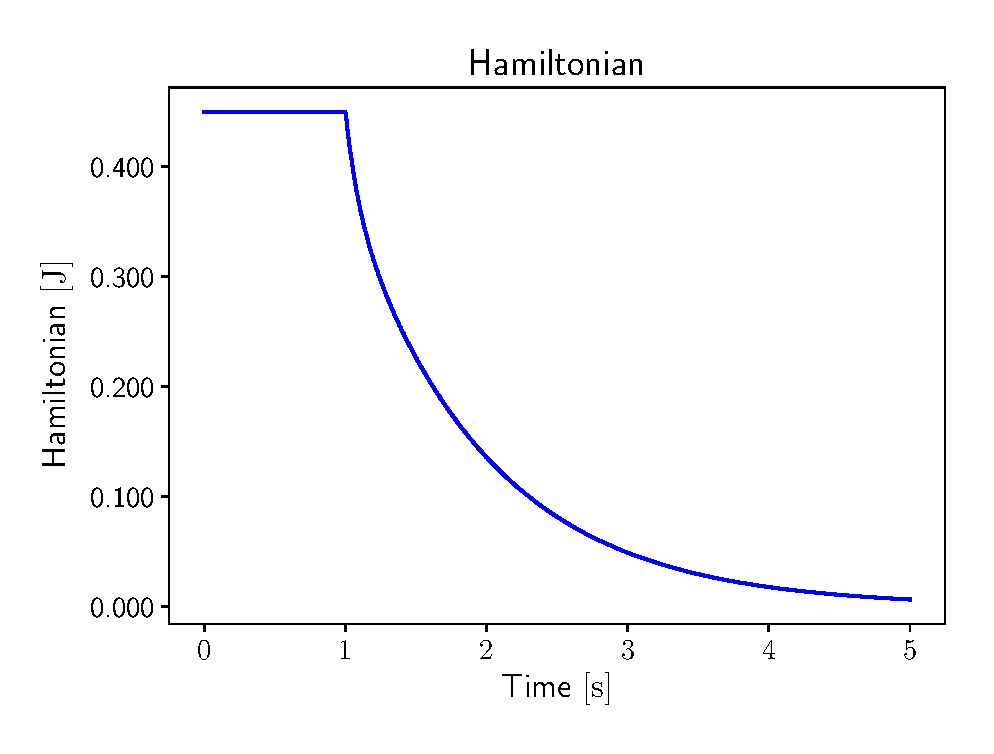
\includegraphics[width=0.7\textwidth]{bs_Kirchh/Hamiltonian.eps}
		\end{figure}
	}
	%\movie[width=0.42\textwidth, height = 0.7 \textheight]{Damped Kirchhoff Plate}{../Videos/Kirchh_Damped_4faster.mp4}
\end{frame}

\section{Conclusion}

\begin{frame}{Open problems and Outlook}
Open problem:
\begin{itemize}
\item \onslide<2->{Finite element space for the Lagrange multiplier, satisfying the inf-sup condition;}
\end{itemize}
	
Developments:
\begin{itemize}
	\item \onslide<3->{Discretization: efficient finite element for the Kirchhoff plate based on div-div conforming elements \footfullcite{chen2020divDiv};}
	\item \onslide<4->{Model reduction: POD methods, $H_2$-optimal strategies or Krilov subspace methods\footfullcite{egger2018};}
	\item \onslide<5>{Observer based boundary control\footfullcite{toledo2020} and reduced LQG design for distributed control\footfullcite{wu2020reduced}.}
\end{itemize}

\end{frame}

\begin{frame}{Additional information}
	
	
Jupiter Notebooks for the wave and heat equation and the Mindlin plate model are available: \\
\vspace{.3cm}
\fullcite{brugnoli2020zenodo}.

\vspace{1cm}

Flexible multibody dynamics for pHs based on the proposed discretization:\\
\vspace{.3cm}
\fullcite{brugnoli2020msd}.

\end{frame}

\end{document}

